\chapter{Valutazione di qualita'}
\label{chap:quality}
Per la misurazione dell'effettiva bontà del nostro sistema di codifica, abbiamo adottato le metriche LPIPS e SSIM \\
Sono entrambe metriche di qualità con riferimento, ergo necessitano di un immagine reference da cui partire e un'immagine obbiettivo su cui calcolare la differenza.\\
La metrica LPIPS si basa sul concetto di perdita percettiva ed effettua una stima istantanea sulla differenza delle immagini; può anche essere migliorato con diverse trasformazioni dell'immagine prima del confronto in modo da essere meno vulnerabile a debolezze di giudizio soggettivo, miglioria che prende il nome di E-LPIPS. \\
E' tuttavia più impreciso di SSIM aggirandosi il punteggio di qualità sempre a circa 170 unità, il che ci rende obbligati ad esaminare molte cifre dopo la virgola.\\
SSIM si basa invece sul concetto di similarità strutturale e al contrario dell'ormai superato PSNR si basa su strutture visibili presenti su un immagine. \\
Effettuando dei test sui video codificati abbiamo stilato una lista di valori di qualità dei video codificati in modo semantico e in modo standard, qualità che si può suddividere in qualità dell'intero video e in qualità delle maschere. Sotto la sperimentazione su 3 video campioni:
\begin{figure}
   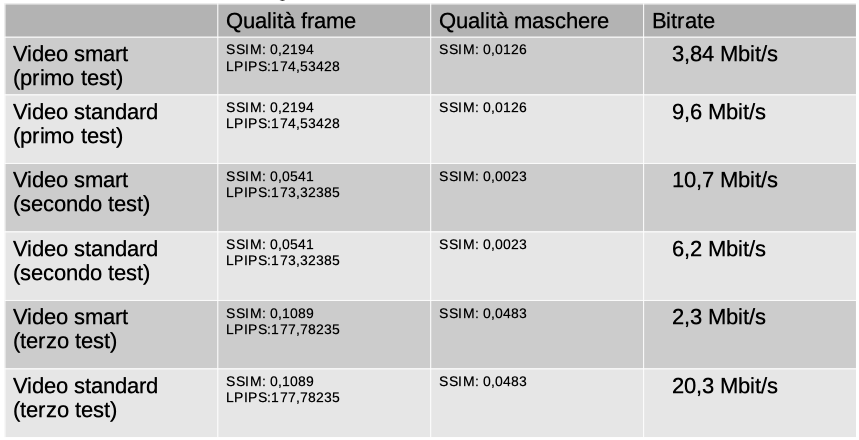
\includegraphics[width=\linewidth]{images/table.png}
   \caption{riassunto valori di qualita'}
   \label{fig:table}
\end{figure}